\chapter{Contexte général de l'étude}

\section*{Introduction}
L’un des critères les plus importants de la réussite d’un projet est la 
satisfaction du client et des utilisateurs finaux. Nous ne pouvons satisfaire
le demandeur sans avoir compris les problèmes qui ont suscité la naissance du projet.
Dans ce chapitre, nous présenterons dans un premier temps la structure dans
laquelle nous avons effectué notre stage. En second lieu, mous parlerons du
projet qui nous a été confié, de son intéret pour l'entreprise, de ses
objectifs et de la problématique y afférente.

\section{La structure d'accueil}

\subsection{Présentation et Histoire}

 \subsubsection{Présentation de la Société Générale Burkina Faso}

 Nous avons effectué notre stage au sein de la Société Générale Burkina Faso \nomenclature{SGBF}{Société Générale Burkina Faso}
une filiale du groupe français \nomenclature{SG}{Société Générale} Société
Générale.
La Société Générale Burkina Faso exerce dans la banque de détail et les services
financiers, la gestion d’actifs et services aux investisseurs et dans la banque
de financement et d’investissement. Elle a pour ambition\footnote{https://societegenerale.bf/fr/votre-banque/presentation}
de:
\begin{itemize}
  \item Bâtir avec ses clients une relation équilibrée et équitable où elle est
    est avec eux , à leurs côtés pour les aider à progresser;
  \item Mettre sa performance au service de ses clients;
  \item Etre la banque relationnelle, référence sur ses marchés, choisie pour la
    qualité et l'engagementde ses équipes;
\end{itemize}

\subsubsection{Historique de la SGBF}

La SGBF a été créée en mai 1998 avec la participation de l'Etat Burkinabé et de
plusieurs partenaires financiers nationaux et internationaux. Elle est née de la 
cession par l’état de $51\%$ du capital de la Banque pour le Financement du Commerce et des
investissements au Burkina (BFCI-B)
\footnote{https://societegenerale.bf/fr/votre-banque/presentation/notre-histoire}.


  \begin{description}
     \item[Septembre 1973:] Création de la Caisse Nationale des Dépots et des
       Investissements(CNDI)\nomenclature{CNDI}{Caisse Autonome des Dépots et des
       Investissements}.
    \item[Août 1984:] Création de l'Union Révolutionnaire de
      Banques(UREBA)\nomenclature{UREBA}{Union Révolutionnaire de Banques}
    \item[Juin 1986:] Création de la Caisse Autonome
      d'Investissement(CAI).\nomenclature{CAI}{Caisse Autonome d'Investissement}
     \item[Août 1986:] Transformation de la CNDI en banque commerciale sous la forme
  d s'une société d'économie mixte.
    \item[Décembre 1987:] Changement de dénomination de CNDI en BFCI-B
    \item[Février 1991 à Décembre 1996:] Mise sous administration provisoire du
  Groupe BFCI-BUREBA-CAI. Fusion-absorption de l'UREBA et de la CAI par 
  la BFCI-B en mai 1995.
    \item[Février 1997:] Cession par l'état de 34\% du capital à des privés
      nationaux.
    \item[Mai 1998:] Cession par l'état de 51\% du capital à des partenaires
      étrangers. La BFCI-B devient la Société Générale des Banques du
      Burkina(SGBB).
    \item[08 février 2013:] Changement de dénomination sociale: la SGBB devient
      la Société Générale Burkina Faso(SGBF).
  \end{description}

  \subsection{Organisation}
   \subsubsection{Organigramme}  
L'organnigramme de la Société Générale Burkina Faso se présente comme suit: 
(voir Figure \ref{fig:organigramme}).
 \begin{figure}[h!]
  \begin{center}
    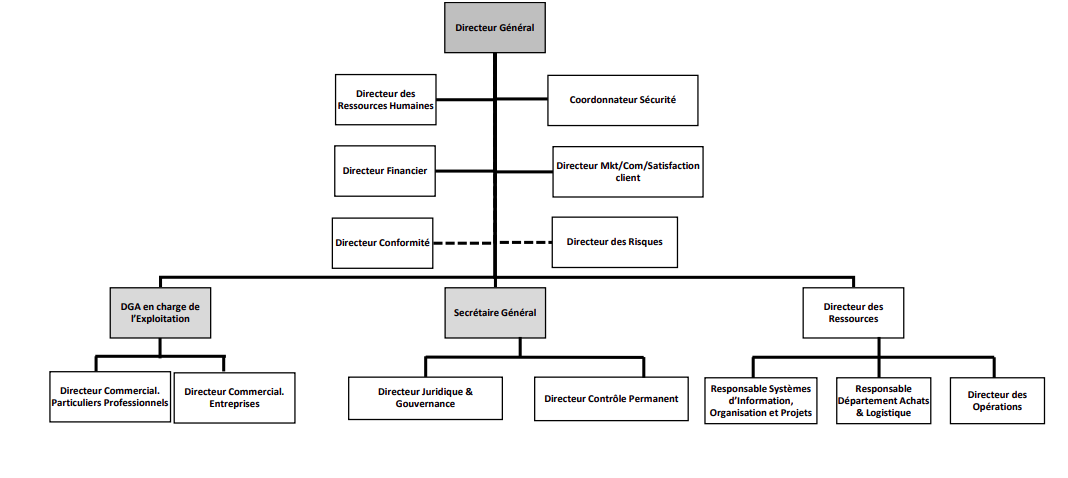
\includegraphics[width=17cm]{images/organigramme.png}
\caption{Organigramme de la société générale Burkina
Faso.\label{fig:organigramme}}
\end{center}
\end{figure}


  \subsubsection{La direction des resources}

Nous avons effectué notre stage au sein de la Direction des Ressources plus précisément
dans la cellule Innovation de cette direction. La Direction des Ressources est 
l’entité chargée de gérer toutes les ressources matérielles et logicielles de la
banque. Les missions de la cellule Innovation, service dans lequel nous avons 
effectué notre stage sont les suivantes:
\begin{itemize}
  \item Continuer de diffuser la culture de l’innovation
  \item Identifier de nouveaux business et services pour les clients
  \item Développer de nouveaux process optimaux dans la réalisation des tâches quotidiennes
    des collaborateurs.
  \item Favoriser l’émergence d’innovations de rupture et tirer parti des technologies et de
    la gestion des données.
\end{itemize}
 
 \section{Présentation du sujet}

\subsection{Libellé du sujet}

\textbf{Application des techniques de Machine Learning à l’analyse de la 
conformité des dossiers de transferts à l'étranger.}

 \subsection{Contexte du sujet}

 L’esprit d'équipe, l’innovation, la responsabilité et l'engagement 
 traversent toutes les activités de la banque.  A travers cette approche,
 la Société Générale cherche des moyens qui lui permettront d’améliorer
 la satisfaction client par un traitement qualitatif et rapide des 
 opérations qui leur ont été soumis. 
 
 Dans ses missions quotidiennes, la SGBF effectue pour ses clients des 
 opérations à l’étranger(pays n'appartenant pas à la zone UEMOA). Ces 
 opérations comportent de nombreux risques de violation des différentes 
 règlementations en cours.

Effectuer une opération de transfert à l'étranger commence par la constitution
d'un dossier appellé dossier de transfert.
Lorsqu’un client veut effectuer un transfert vers un pays  étranger, la
règlementation exige qu’il transmette à l’intermédiaire agréé qui est la banque
un certain nombre d’éléments permettant de justifier le transfert qu’il voudrait
initier. L'ensemble de ces éléments constitue le dossier de transfert. L’analyse
du dossier par les experts de la règlementation s’effectue après que le client 
soit reparti. Une journée complète peut s'écouler entre le moment où le dossier
est déposé au guichet et celui où le transfert est réellement effectuer et ceci 
lorsque le dossier ne comporte aucune irrégularité. 

En cas d’irrégularités, le dossier est transmis au conseiller du client qui se 
chargera de le contacter pour lui demander de passer corriger les irrégularités
qui ont été constatées sur son dossier. Lorsque les irrégularités ont été
corrigées, le dossier reprend le circuit d'analyse.

Dans un domaine où la satisfaction du client et la célérité dans le 
traitement des opérations est une exigence et face à l'augmentation 
significative des règlementations et obligations de communications qui en
découlent, vingt-quatre heures pour traiter une opération est un délai déjà
long. Lorsque le dossier comporte des irrégulariés ce délai sera encore
rallonger d'au moins 24 heures encore. 

Lorsque un dossier non conforme à la conformité passe malgré le système d'analyse
mis en place par l'institution financière en l'occurance la SGBF ce sont 
d'importantes sanctions financières et disciplinaires qui lui seront imposées.
En 2018 par exemple, la SG a payé une amende d'environ 1.2 milliards d'Euros 
pour des opérations en dollars vers des entités sanctionnées par les autorités 
américaine.

Au vue des enjeux économiques que suscitent ces situations, nous nous sommes 
posés la question comment permettre aux collaborateurs du services Opérations
Internationales(OPI) \footnote{Le service OPI est un service appartenant à la
direction des Opérations(DOPE)}
\nomenclature{OPI}{OPérations Internationales} de donner à un client l’état de son opération
vis à vis de la règlementation sous réserve d'un contrôle beaucoup plus approfondi. 
Cela permettra d'une part de diminuer la charge de travail des collaborateurs de la banque
et rassurera d'autre part le client sur la volonté des collaborateurs de 
traiter diligemment de son opération.

\subsection{Intérêt du sujet}
 
Ce projet est d’un intérêt très élevé pour la SGBF car elle vise à
apporter des solutions pour le traitement rapide des opérations à l'étranger.
Les résultats attendus sont:
\begin{itemize}
  \item Un gain en temps,
  \item Une facilité de prise de décision,
  \item Une grande disponibilité et de performance 
  \item Un système toujours actuel et compatible
  \item Faciliter la gestion des réclamations
\end{itemize}

    \subsection{Problématique du sujet}

Le service des opérations internationales (OPI) reçoit en moyenne quatre-vingt-dix
(90) dossiers d’opérations de transferts par jour. Ces opérations sont de
plusieurs types et comprennent transactions quotidiennes, périodiques et 
apériodiques effectuées par, ou touchant à de nombreuses parties prenantes
telles que les employés, les clients, les débiteurs et des entités externes.
La nature complexe de ces activités et de ces activités et transactions 
nécessite une surveillance constante pour s’assurer que ni la banque, ni
ses employés ne sont exposés à des risques.

Une analyse rigoureuse est donc appliquée après réception d’un dossier au guichet.
Cette analyse concerne aussi bien les différents intervenants de l'opération que
la nature l'opération elle-même.
Cette analyse peut être décrite suivant trois axes majeurs :
\begin{itemize}
  \item Analyse de la complétude du dossier 
  \item Analyse de la fiabilité des différents intervenants de l'opération 
  \item Analyse de la conformité règlementaire de l'opération
\end{itemize}
C'est après toutes ces analyses que le dossier est transmis pour saisie et
validation dans  le CBS\nomenclature{CBS}{Core Banking System}. Si le dossier comporte des 
irrégularités, il est transmis au conseiller ou à la conformité pour demande
d'accord. Sinon la saisie est validée et le transfert éffectué.

Pour pouvoir mettre en place un système qui puisse analyser les dossiers de ces
opérations, il nous faudra trouver des réponses aux questions suivantes:
\begin{itemize}
  \item Comment codifier le dossier d'une opération à l'étranger ?
  \item Quels sont les caractéristiques qui entre en jeux dans l'analyse d'un
    dossier de transfert ?
  \item La règlementation financière est un outil  qui évolue. Comment mettre en
    place un système qui puisse très vite s'adapter à des évolutions ?
  \item La Banque a l'obligation de communiquer avec le client sur la raison
    pour laquelle son opération a été rejetée au cas où elle l'est. Quels 
    méthodes d'apprentissage sied le mieux à ce problème ?
\end{itemize}
Pour répondre à ces interrogations, nous allons explorer tous les contours du
domaine d'étude, afin de fixer les bases solides qui nous permettront de mener
notre projet à son terme.

\subsection{Objectifs}

L’objectif de l’étude est de développer un environnement permettant une analyse des dossiers et des 
intervenants des différentes opérations de transferts.
Spécifiquement, il s'agit de 
\begin{itemize}
\item comprendre le processus d'analyse de dossier afin de dégager les grandes étapes;
\item Proposer un modèle de machine learning permettant d'analyser un dossier de
  transfert fourni en paramètre vis à vis de la règlementation;
\item Utiliser le modèle qui aura été mis en place afin de détecter des
  transactions suspectes;
\item Mettre en place une interface web permettant d'utiliser ce modèle.
\end{itemize}

\section{Traitement des données et formats de fichiers}

TECHNI DRONE utilise plusieurs logiciels pour le traitement des donnéées après
les campagnes d'acquisition faites par drones. Cette etape est tres importante 
dans la mesure ou elle aboutie à la realisation des carte representant une carriere.

\begin{figure}[h]
  \begin{minipage}[c]{.46\linewidth}
      \centering
      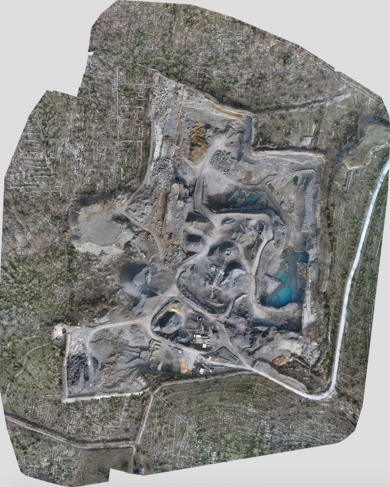
\includegraphics[width=8cm, height=8cm]{images/orthomosaique.png}
  \end{minipage}
  \hfill%
  \begin{minipage}[c]{.46\linewidth}
      \centering
      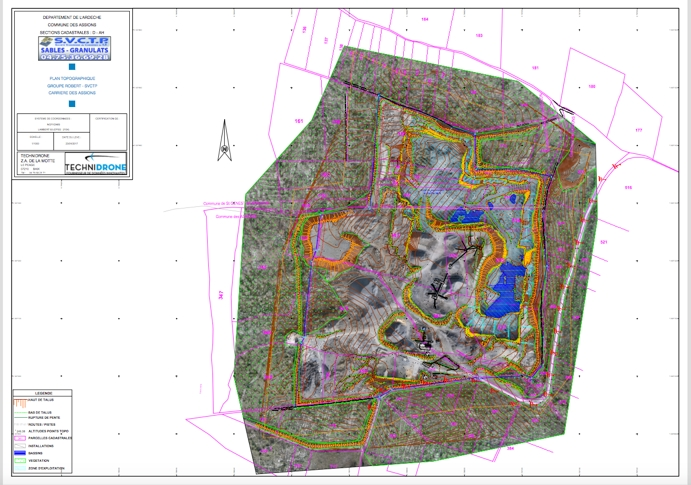
\includegraphics[width=8cm,height=8cm]{images/carteCarriere.jpg}
  \end{minipage}
  \caption{L’ortho mosaïque de la carrière et la carte de la carrière.
     \label{fig:credit}}
\end{figure}

\subsection{Pix4D}

Le traitement des images acquisent par drones est fait avec le logiciel Pix4D.
Pix4D est un logiciel de photogrammétrie pour la cartographie professionnelle 
basée sur des images de drones uniquement. 
\begin{figure}[h]
  \begin{center}
    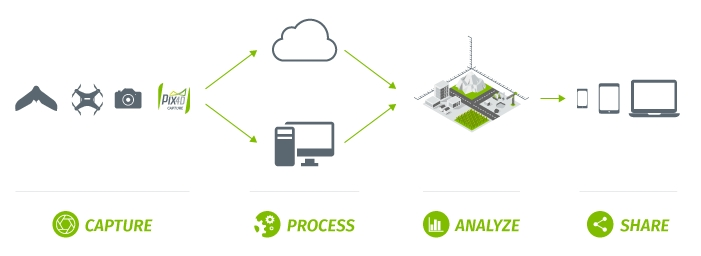
\includegraphics[width=12cm]{images/processusPix4D.jpg}
     \caption{Processus de traitement Pix4D.
     \label{ProcesPix4D}}
  \end{center}
\end{figure}
Le logiciel convertit les images 
aeriennes prise par drones en orthomosaiques 2D georeferencées, en model 
surface 3D texturé et en nuages de points. ce processus prend environ une dizaine
d'heures comment le montre la Figure~\ref{ProcesPix4D}. 

Dans la Figure~\ref{positionImage}, les points rouges representent les positions
des images prises drone et Les croix bleues sont les points GCPs
(Group Control Point)\footnote{Les GPCs sont des 
marqueurs visuels sur le sol avec des coordonnées connues qui augmentent 
la précision ortho mosaïque et permettent l'alignement de plusieurs 
campagnes d’acquisition.}. Le logiciel utilise les coordonnées des ces point
pour faire le recalage des images et produit les nuages de point et le maillage 3D
de la carrière. Le logiciel met aussi à disposition des outiles pour la detection
manuel des ligne de ruptures de pente directement sur les nuages de points ou
sur le maillage 3D. Les coordonnées de ces ligne ainsi detecter sont enregistrer
dans un fichier au format shapefile(.shp)\footnote{Shapefile est un format
de fichier ouvert compatible avec le logiciel OpenSource QGIS}. Cette phase
d'annotation prend egalement une dizaine d'heure pour un employé habitué au logiciel.
La Figure~\ref{annotationMallage} montre triangulaire 3D créé par pix4D,
sur lequel se basé pour détecter les lignes de ruptures de pente.

\begin{figure}[h]
  \begin{center}
    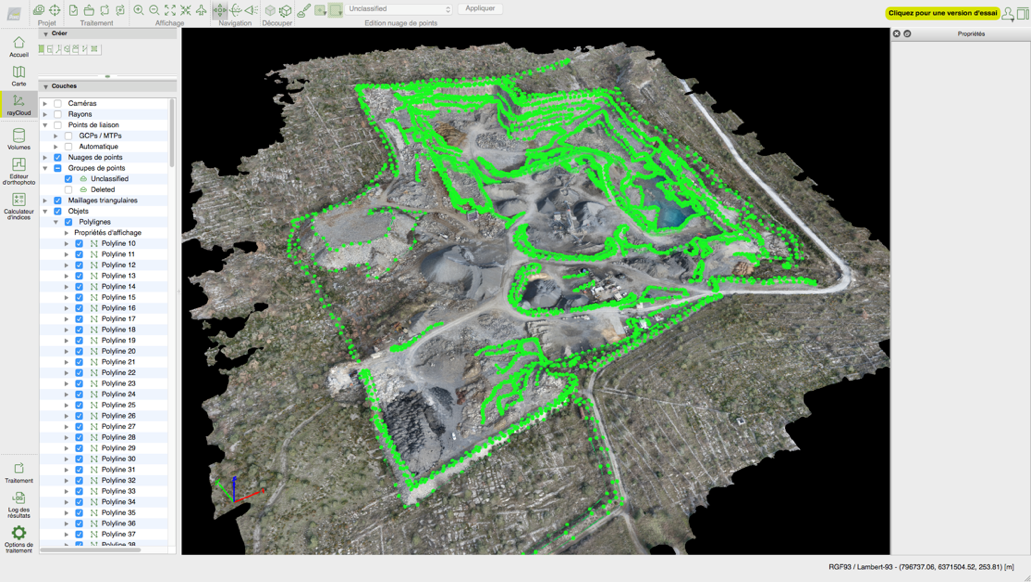
\includegraphics[width=12cm, height=5cm]{images/detctionLigne.jpg}
     \caption{Detection manuel des lignes de ruptures de pente.
     \label{detctionLigne}}
  \end{center}
\end{figure}
\begin{figure}[h]
  \begin{center}
    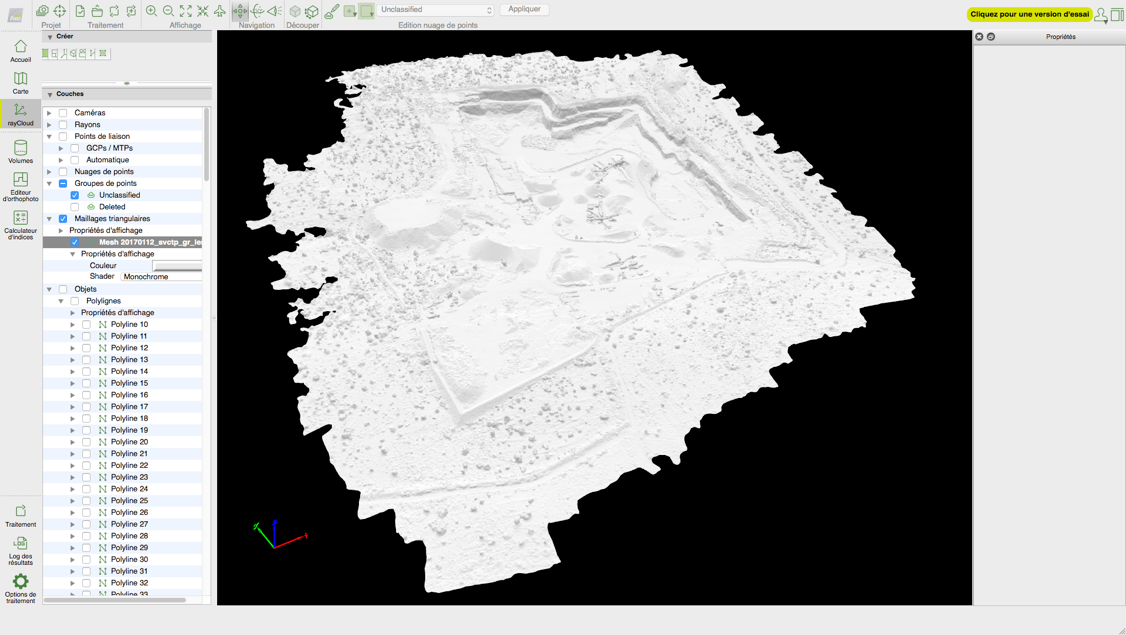
\includegraphics[width=12cm,height=5cm]{images/maillageSansTexture.jpg}
     \caption{Maillage 3D sans texture.
     \label{maillageSansTexture}}
  \end{center}
\end{figure}
\begin{figure}[h]
  \begin{center}
    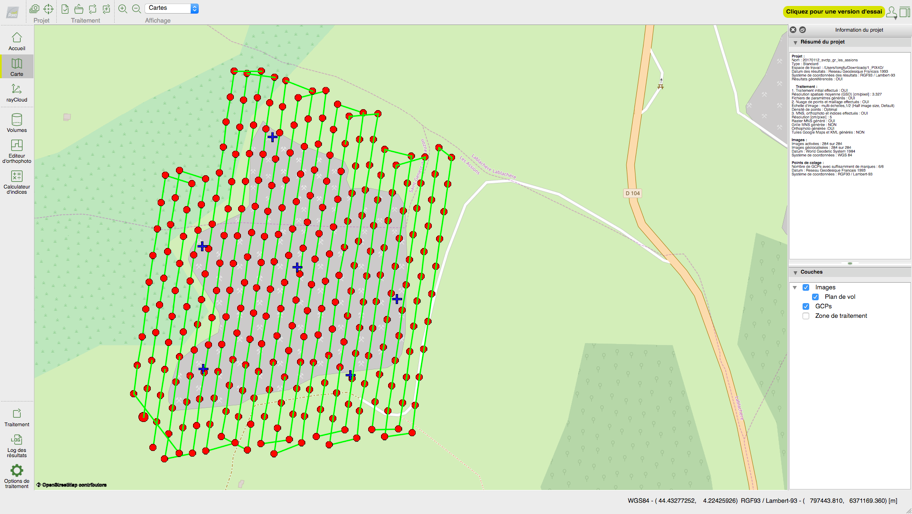
\includegraphics[width=12cm]{images/positionImagePix4D.jpg}
     \caption{Position des images prise par drones.
     \label{positionImage}}
  \end{center}
\end{figure}

\subsection{QGIS}

QGIS est un logiciel SIG (système d'information 
géographique) libre multiplate-forme publié sous licence GPL. 
il gère les formats d’image matricielles (raster) et vectorielles,
ainsi que les bases de données [Wikipedia](https://en.wikipedia.org/wiki/)\dots
TECHNI-DRONE utilise ce logiciel pour classifier les lignes de 
ruptures de pente par rapport aux courbes de niveau.
\begin{figure}[h]
  \begin{center}
    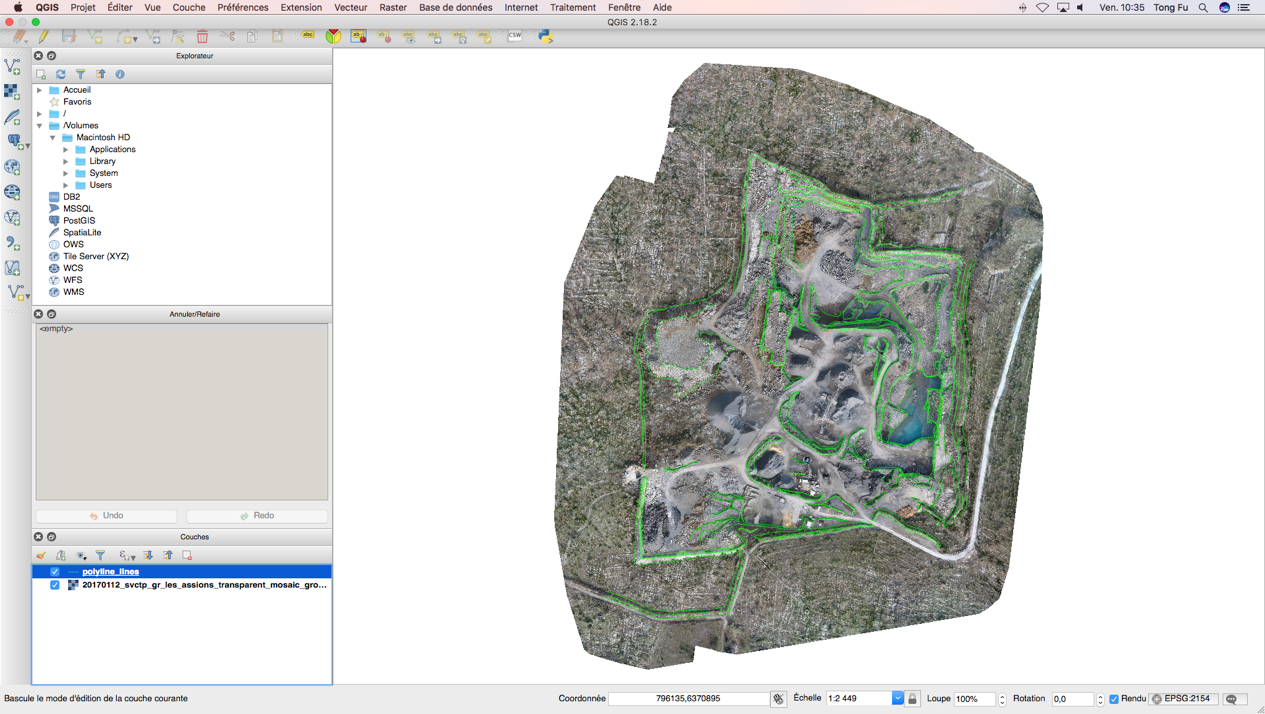
\includegraphics[width=12cm]{images/QGIS.jpg}
     \caption{Classification sur QGIS.
     \label{QGISClassification}}
  \end{center}
\end{figure}


\section*{Conclusion}
Il  a été question dans ce chapitre de présenter  la structure d’accueil,
la SGBF, qui a suivi et coordonné tous les travaux .Ensuite nous avons
présenté le sujet qui nous a été confié, dégager sa problématique et
l’intérêt qu’il suscite pour la Société Générale Burkina Faso. Dans la suite,
il sera question  d’aborder le machine learning et les algorithmes de classification.
